\section{Performance Evaluation} %Overhearing Experiments}
\label{sec::OverhearingExperiments}
%


%In this section, we first describe the experiment settings and then show the
%our simulation settings about how we
%generate the testing images and then give some discussions about the experiment
%evaluation results for the algorithm proposed in Section~\ref{sec::SchedulingAlgorithm}.

\subsection{Experiment Settings}
\label{sec::ExperimentSettings}

To create quasi-realistic $3$D city views, we make use of an open-source
%To show the advantage of overhearing source coding in the wireless multimedia
%sensor network under a more realistic scenario, we make use of an open source
$3$D modeling software~\cite{Blender} and a $3$D city generator~\cite{Suicidator}.
%called suicidator~\cite{Suicidator}.
%Create detailed city backgrounds
%Blender is a powerful $3$D modeling software that we can use it to generate
%$3$D objects.
%We can use a python script to control the position of all these $3$D objects in
%Blender as well as the lighting source.
%Therefore, we can create a more realistic city scene and make our experiment
%more practical.
%Besides, we also use a free
%A Blender addon called suicidator~\cite{Suicidator} is also used
%to generate a $3$D city for installing camera at crossroads.
%The free version of suicidator can generate a city with size $500 m^2$.
%By setting different parameters in suicidator, we can create a different city
%view.
%For example, we can change the density of streets so that the city looks more
%crowded, and we can also change the texture of buildings to make the city
%different.
A total of $30$ cameras are then deployed at different locations (crossroads)
inside the city of size $500 m^2$ (limited by the capacity of the modeling software)
%After creating these objects, Blender allows us to install cameras at a target
%position and a fixed sensing direction for collecting testing images.
for collecting the desired city snapshots (${1280 \times 720}$ HD images).
Then, H.264~\cite{JMVC} is used to encode the images
collected by individual cameras with or without reference frames.
% to analysis the correlation
%
%Besides, we also use a free Blender addon called suicidator~\cite{Suicidator}
%to generate a $3$D city for installing camera at crossroads.
%The free version of suicidator can generate a city with size $500 m^2$.
%By setting different parameters in suicidator, we can create a different city
%view.
%For example, we can change the density of streets so that the city looks more
%crowded, and we can also change the texture of buildings to make the city
%different.
%Therefore, by using Blender and suicidator, we can collect various scenes to
%verify our proposed algorithm under a more realistic scenario.
%The steps of our experiment settings is summarized as follows:
%\begin{enumerate}
%\item Create a $3$D city in Blender using the suicidator addon.
%\item Install $30$ cameras at different crossroads of the $3$D city.
%\item Collect images from those cameras.
%\item Use a H.264 reference software~\cite{JMVC} to analysis the correlation
%between cameras.
%\end{enumerate}
%
Figure~\ref{fig::cityAndCamera} shows the $3$D city view and the deployment
locations for $30$ cameras.
%our camera deployment in Blender.
With reference to real-world applications,
%~\cite{CameraInstallation}, multiple
multiple cameras are deployments at one crossroad for capturing views from different angles.
The arrow in Figure~\ref{fig::cameraDeployment} is the sensing direction of
each camera while different groups of cameras are shown by different colors.
%(purple color are used for cameras which has not been grouped with other
%cameras).
%Note that we might install more than one camera at a crossroad since some of
%the real-world WMSN applications do so~\cite{CameraInstallation}.
%Each camera is responsible for collecting images for their own area of
%interest (determine by its position and sensing direction).
%To proceed, we now show how we install cameras at a given crossroad.
\ignore{
Figure~\ref{fig::crossroadCamera} gives one group of $3$ cameras deployed at one
crossroad, and
%Suppose at some of the crossroads in the city, we install $3$ cameras and each
%camera has its own sensing direction, the position of cameras is similar to the
%deployment shown in Figure~\ref{fig::crossroadCamera}.
%Obviously, the scenes of these $3$ cameras at the same crossroad is correlated
%with each other since there exists some overlap of their area of interest.
Figure~\ref{fig::testImages} shows the collected images of the $3$ cameras.
%camera deployment of Figure~\ref{fig::crossroadCamera}.
%
It can be observed that images collected by different cameras are highly correlated,
especially for those at the same crossroad, due to the overlap in the view angles.
%We can see in Figure~\ref{fig::testImages} that there exists some similarity
%between collected images at the same crossroad.
%Therefore, the total encoded bits can be reduced if we make use of this
%correlation in a proper way.
}
{\color{blue}

Based on the above settings, we can obtain the amount of encoded bits
(${H(X_1), H(X_2), \cdots H(X_{30})}$) of each camera by independent encoding
its snapshot (${X_1, X_2, \cdots X_{30}}$) through the H.264 reference
software.
The correlation between two cameras (${H(X_i|X_j),i\neq j,1\leq i,j\leq 30}$)
is then analyzed by the multiview encoding of two different snapshots.
Therefore, we can generate a correlation matrix $\mathcal{H}$ where the $i-j$
entry of $\mathcal{H}$ is $H(X_i|X_j)$.
The correlation matrix $\mathcal{H}$ can be further used for our scheduling
algorithm described in Section~\ref{sec::SchedulingAlgorithm}.
}

\begin{figure}[t]
\begin{center}
\begin{subfigure}[b]{0.9\columnwidth}
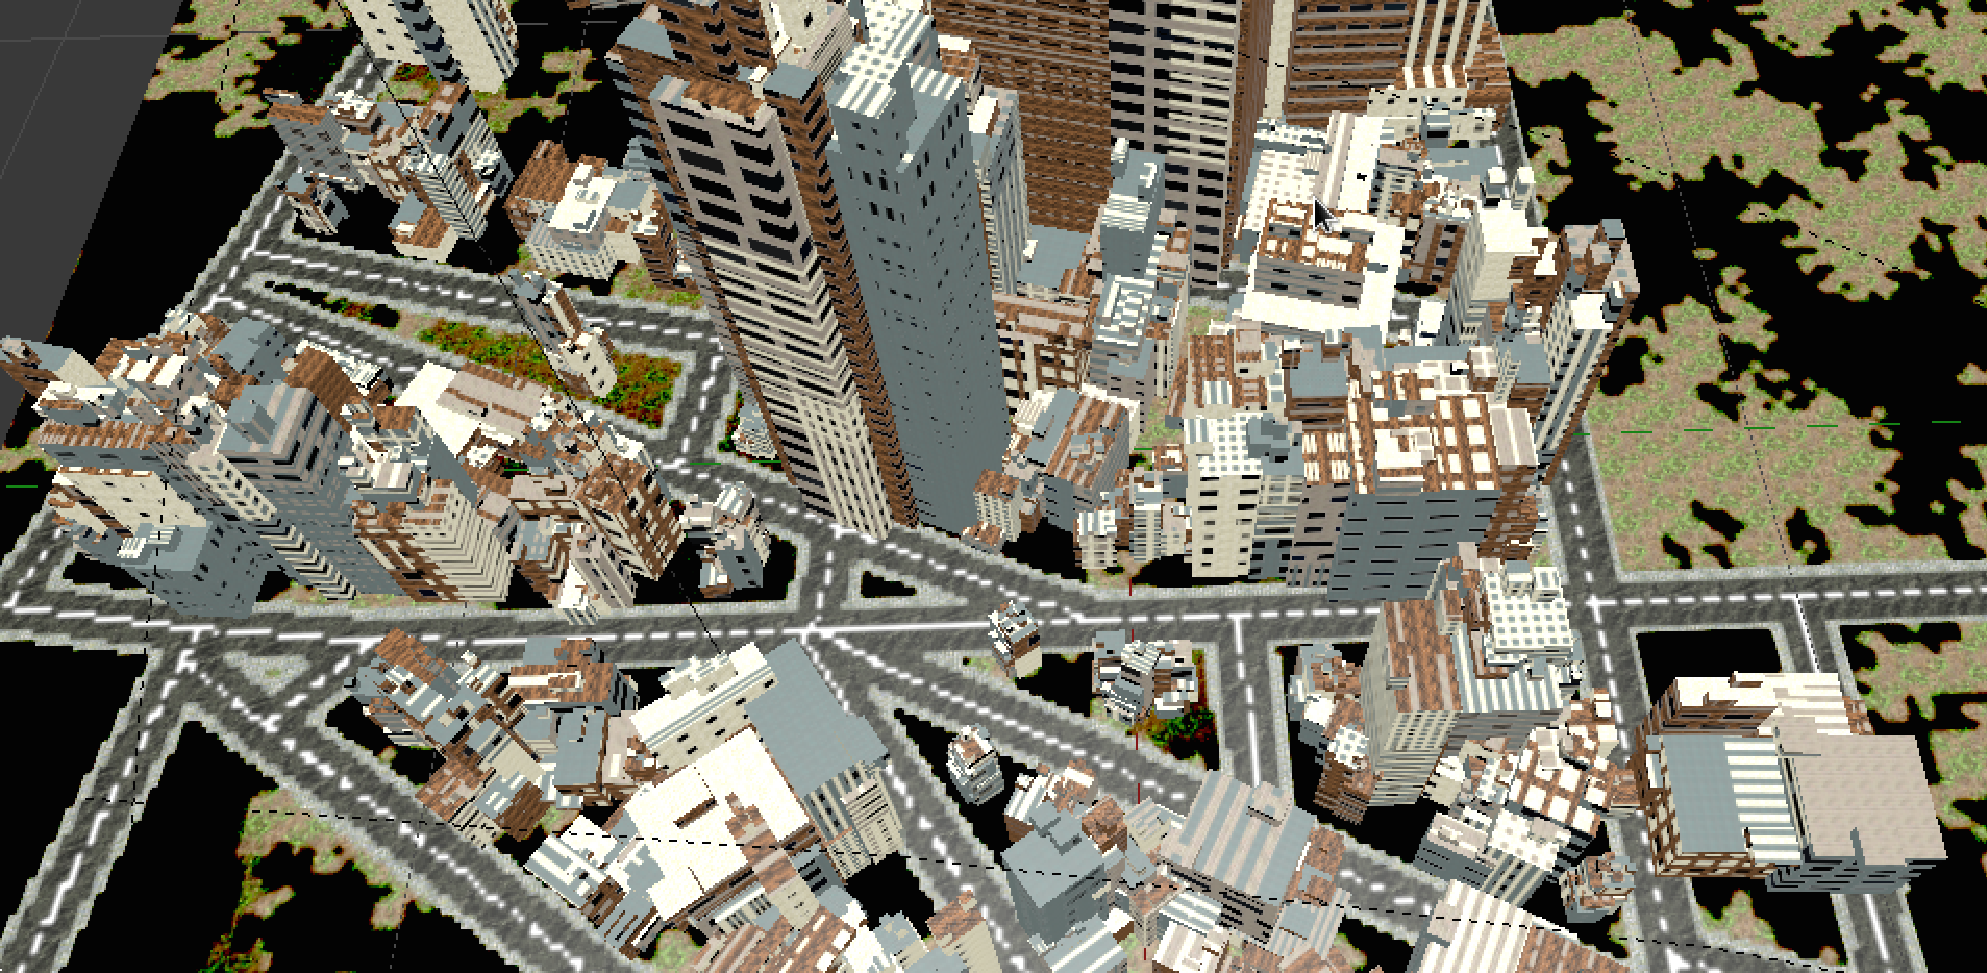
\includegraphics[width=0.9\columnwidth]{./fig/cityView.pdf}
\caption{\label{fig::cityView}City view}
\end{subfigure}
\hfill
\begin{subfigure}[b]{0.9\columnwidth}
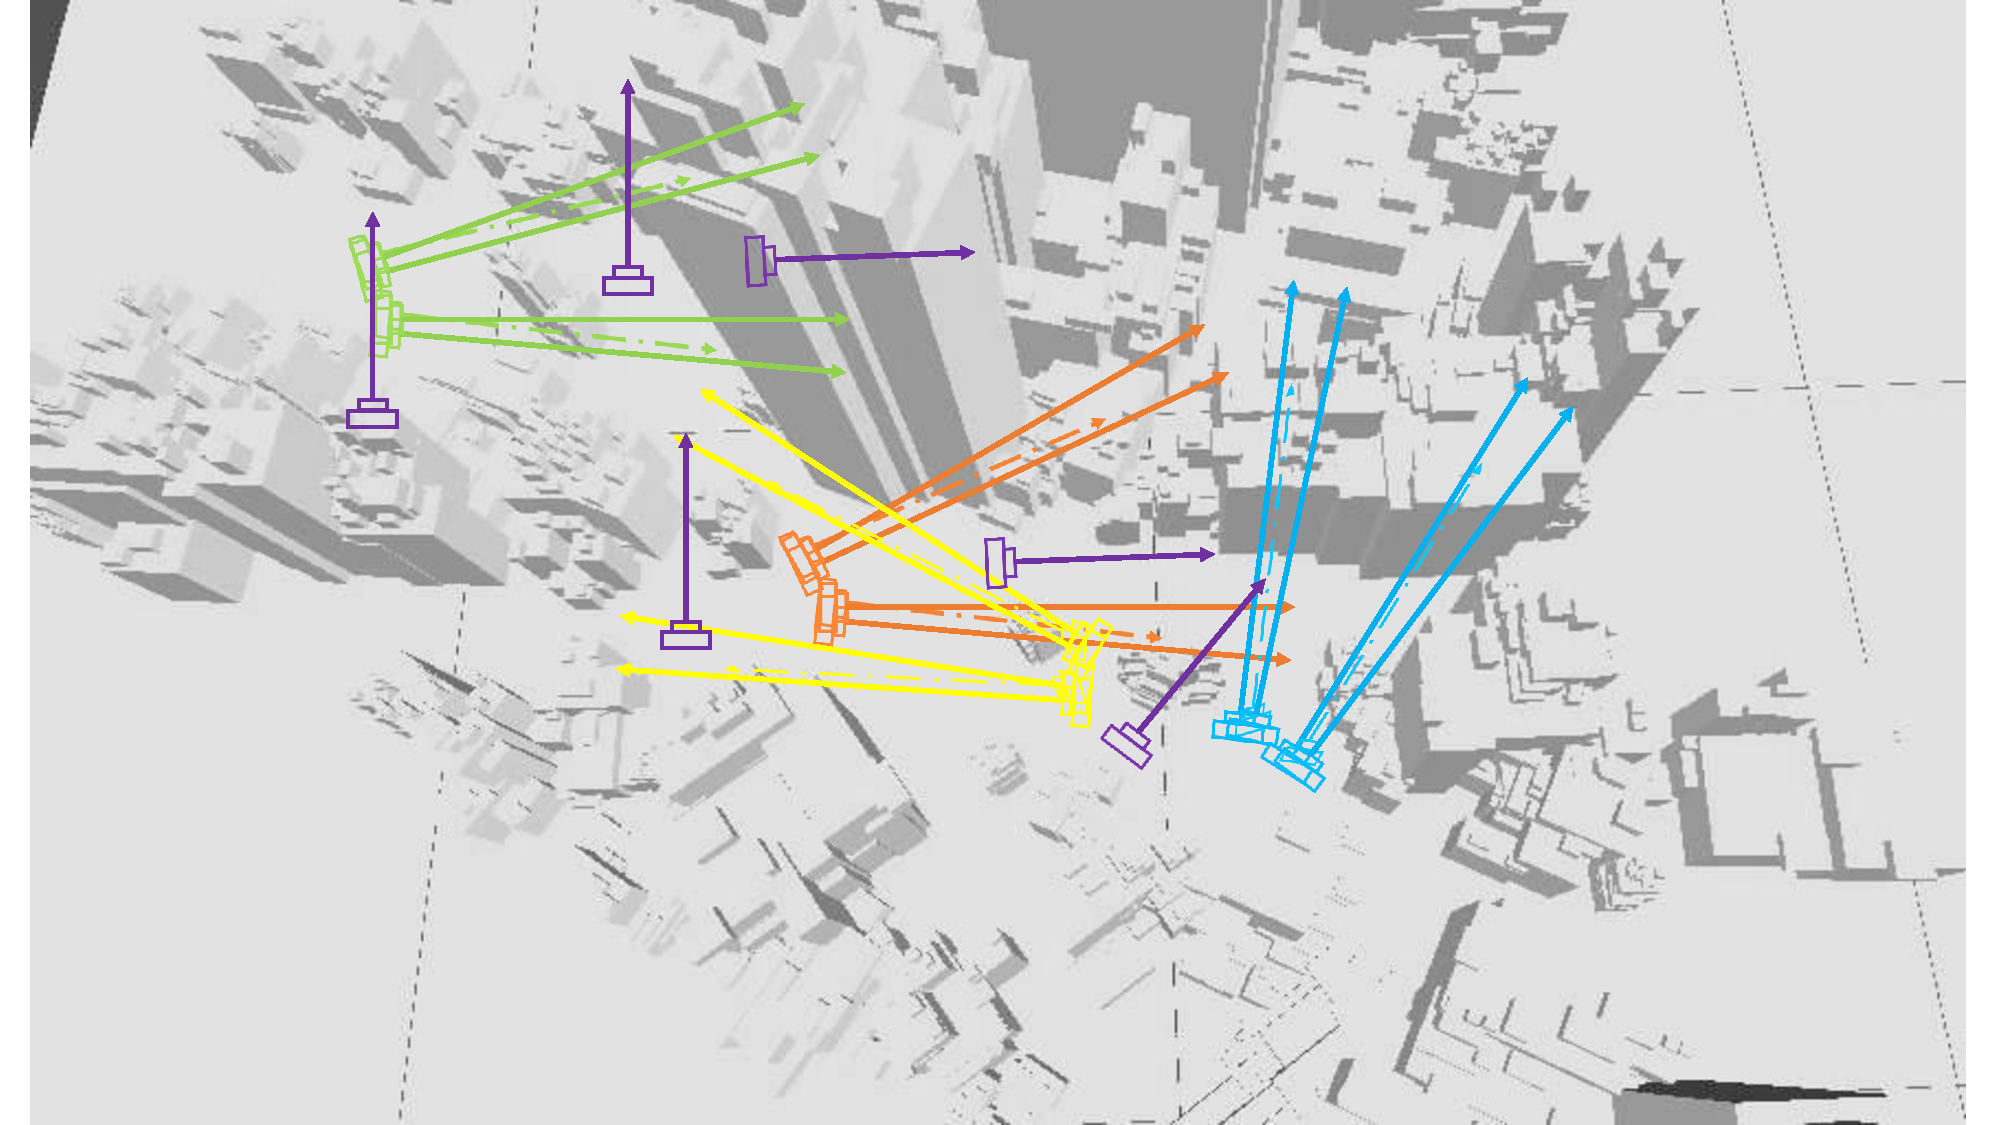
\includegraphics[width=0.9\columnwidth]{./fig/newCameraDeployment.pdf}
\caption{\label{fig::cameraDeployment}Camera deployment}
\end{subfigure}
\caption{\label{fig::cityAndCamera}City view and camera deployment}
\end{center}
\end{figure}

\ignore{
\begin{figure}
\begin{center}
\begin{subfigure}[b]{0.95\columnwidth}
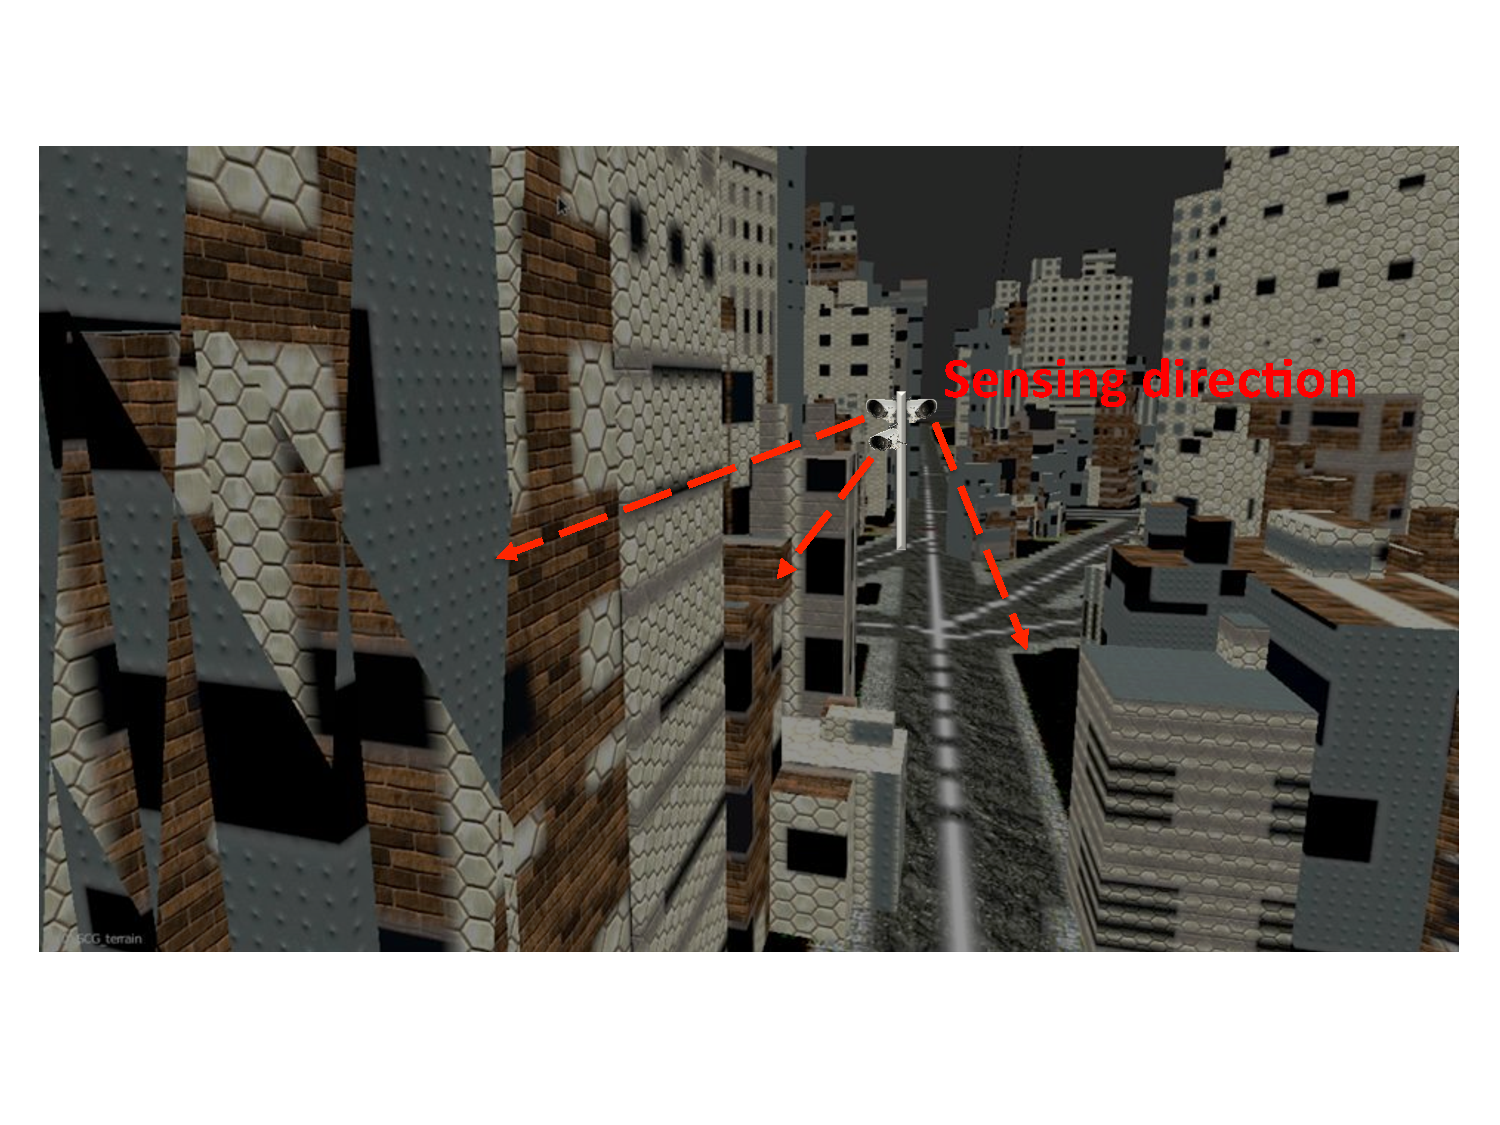
\includegraphics[width=0.95\columnwidth]{./fig/cameraAtCrossroad.pdf}
\caption{\label{fig::crossroadCamera}Camera deployment}
\end{subfigure}
\hfill
\begin{subfigure}[b]{0.95\columnwidth}
\includegraphics[width=0.95\columnwidth]{./fig/imageAtCrossroad.pdf}
\caption{\label{fig::testImages}Testing images}
\end{subfigure}
\caption{\label{fig::givenCrossroad}Camera deployment and collected images at a
given crossroad}
\end{center}
\end{figure}
}
%

\subsection{Dominating Set Problem Evaluation}
\label{sec::DSEvaluation}
\begin{figure}
\begin{center}
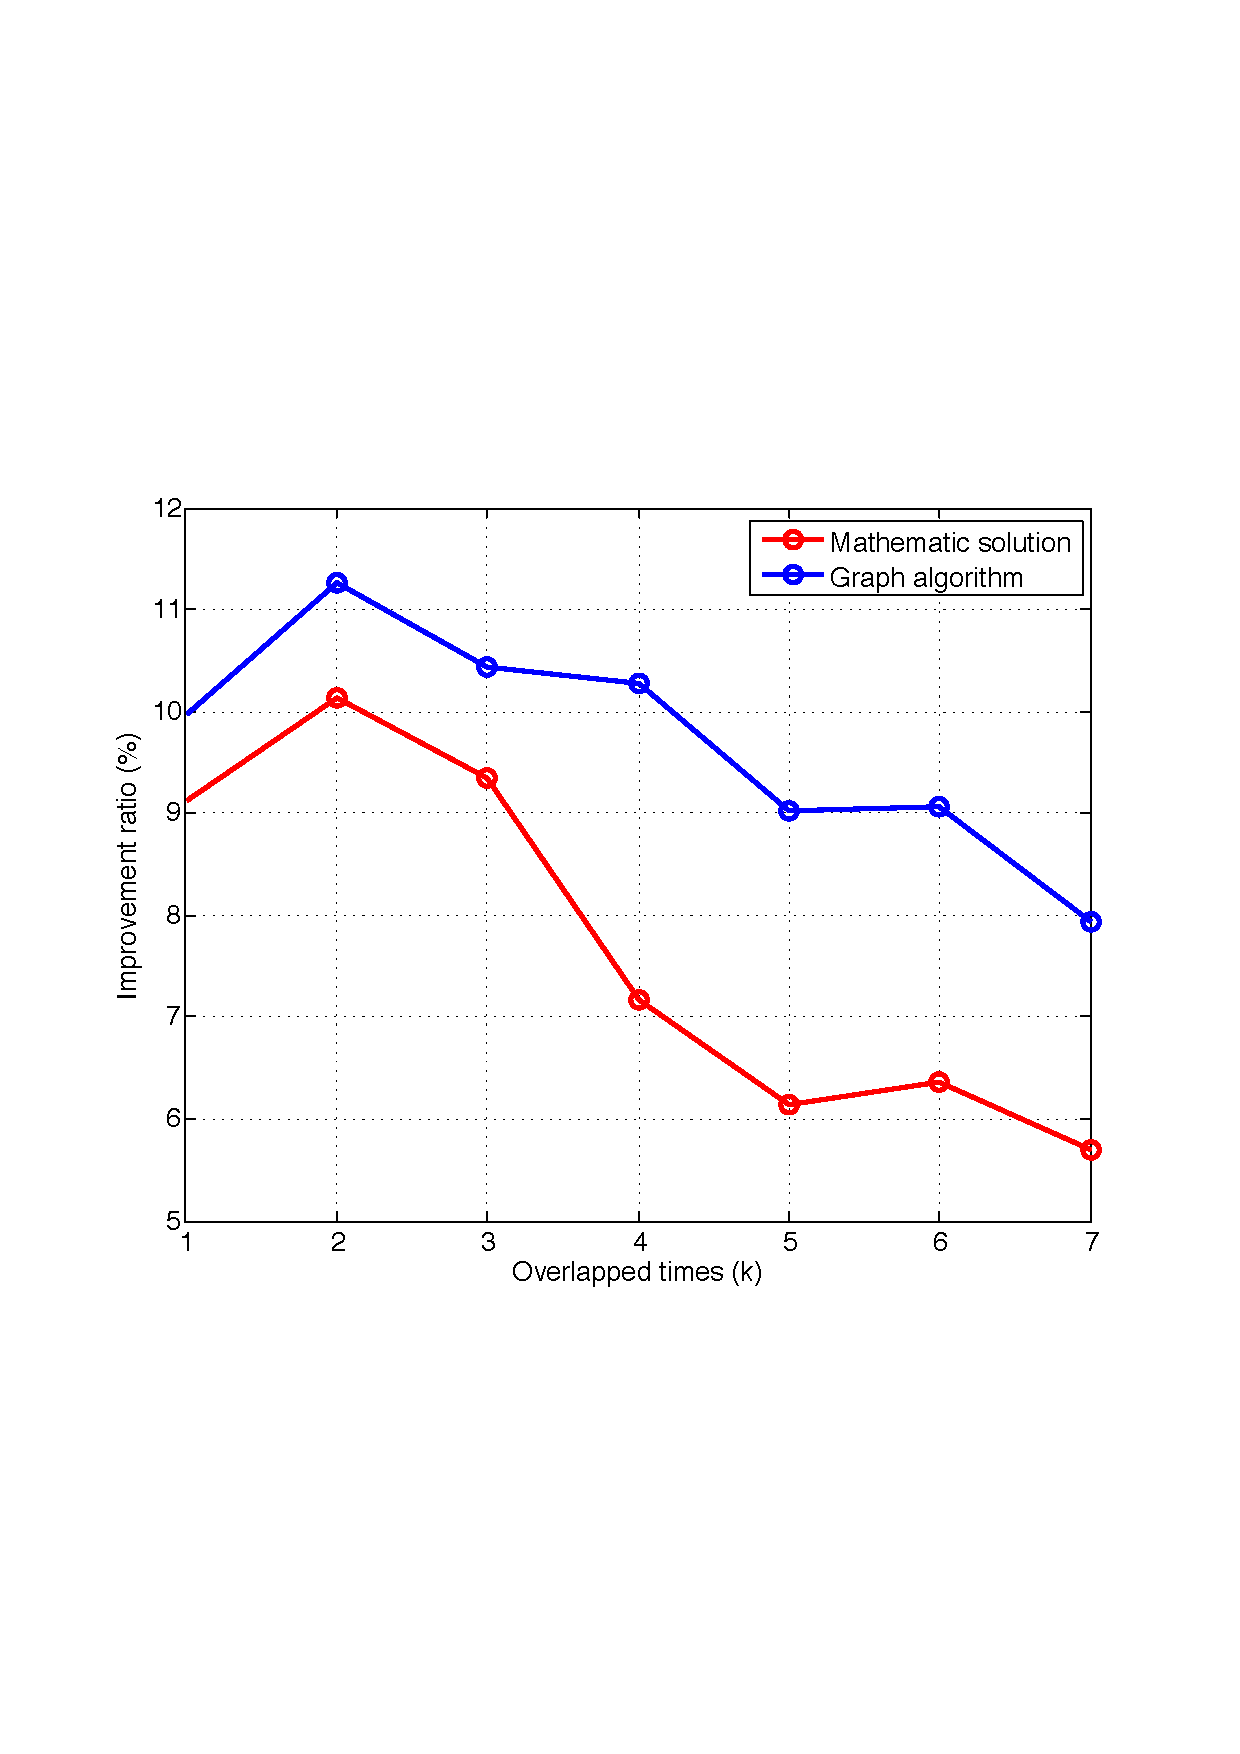
\includegraphics[width=0.9\columnwidth]{./fig/compareDSAlgorithm.pdf}
\caption{\label{fig::overlapped} Number of candidate reference broadcasters}
\end{center}
\end{figure}
{\color{blue}
As we mentioned before, changing the value of $k$ in
Problem~\eqref{eq::relaxedMDS} will cause a difference in the system
performance.
We here increase the value of $k$ from $1$ to $7$ and compare the mathematic
solution versus the heuristic graph algorithm.
The results is shown in Figure~\ref{fig::overlapped} and we can learn that
$k=2$ is the best choice in our network scenario.
This is because $k=2$ tends to select a proper amount of broadcasters for
independent transmission.
Therefore, if we increase the value of $k$ becomes larger than $2$, it happens
that there are too many independent transmitters and the advantage of
overhearing is not that evident.
However, we still want to argue that if the network becomes larger, increasing
the value $k$ is necessary to keep the overhearing performance.
}

\subsection{Experiment Results}
\label{sec:ExperimentResults}

\begin{figure}
\begin{center}
%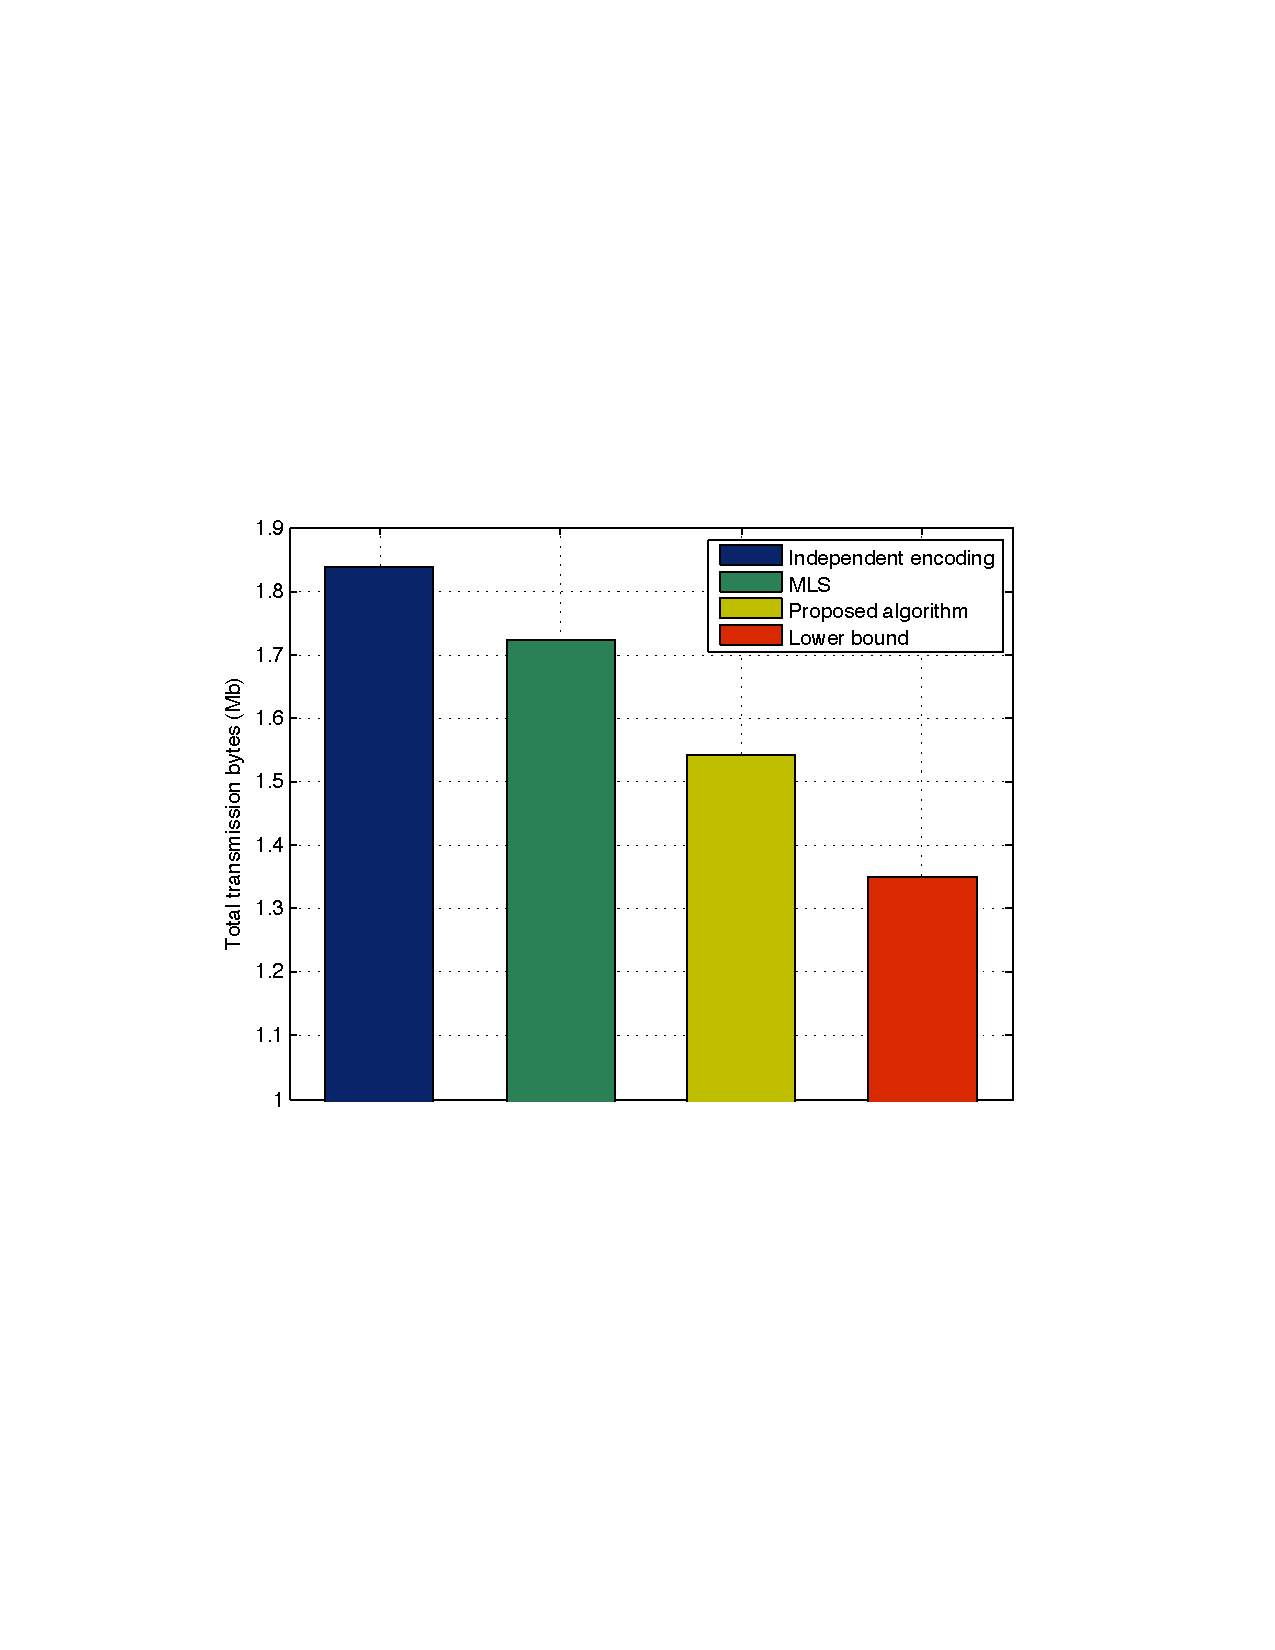
\includegraphics[width=0.95\columnwidth]{./fig/transByte.pdf}
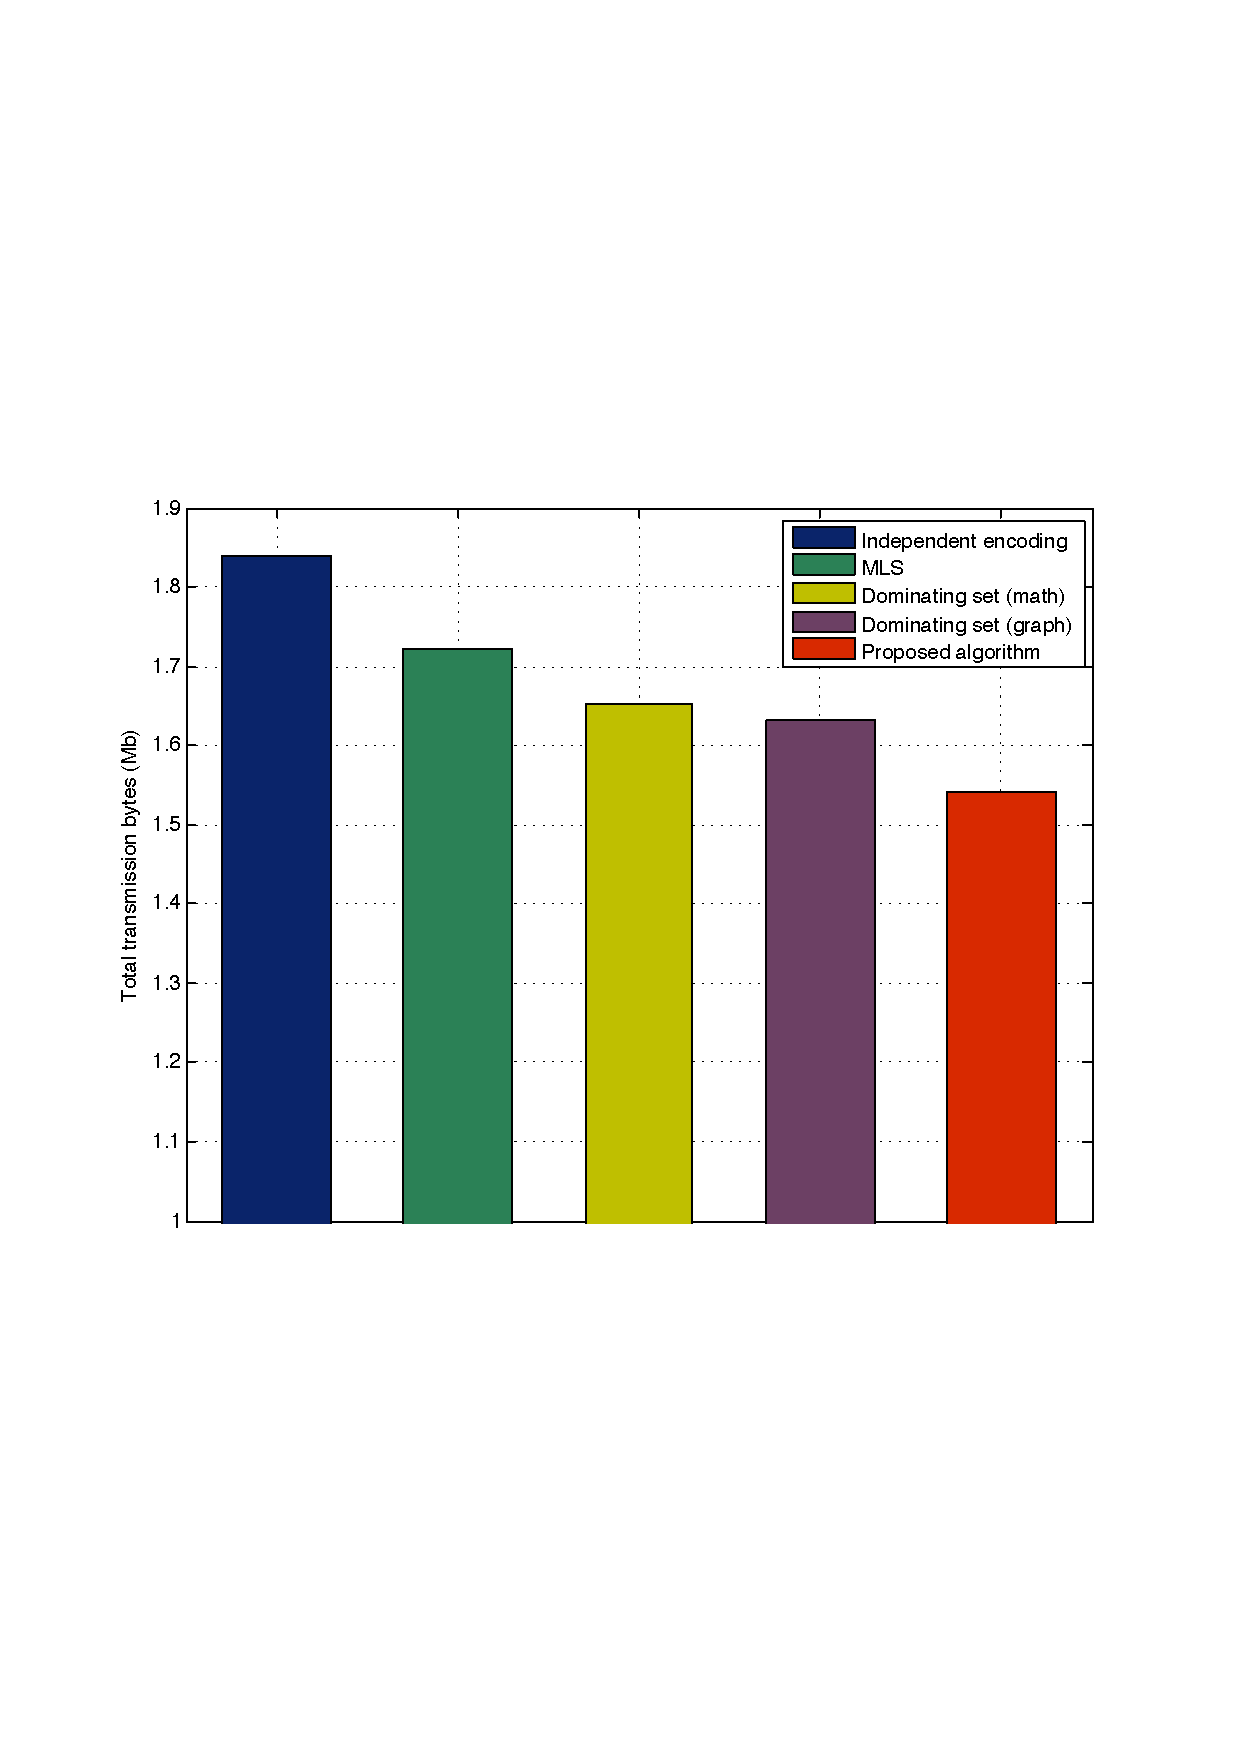
\includegraphics[width=0.9\columnwidth]{./fig/transByte5.pdf}
\caption{\label{fig::transByte}Performance comparison}
\end{center}
\end{figure}

%By using the experiment settings described in
%Section~\ref{sec::ExperimentSettings}, we show our experiment results about
%the total required encoded bits in this section under the image resolution of
%${1280 \times 720}$.
To evaluate the performance of the proposed algorithm, we compare against the
MLS algorithm proposed in~\cite{MLS}.
%the performance of our proposed algorithm with the MLS (maximum
%lifetime scheduling) problem, which has been well investigated in~\cite{MLS}.
The authors in~\cite{MLS} solve a {\em relaxed integer programming} problem to obtain
the probability that a camera should overhear transmissions of other cameras.
%of a camera should whether overhear others' transmission or
%transmit independently.
Since the binary decision for each camera is made by approximating the probability
thus solved,
%However, their approximation algorithm for transforming the obtained
%probability into an integer value seems too conservative.
there is performance loss during the transformation.
%That is, there might be too many cameras perform independent encoding, causing
%an inefficient usage of the limited radio resource.
%
Figure~\ref{fig::transByte} shows that MLS can improve the baseline performance
(all cameras perform independent encoding) for $6.3 \%$,
%shows that the improvement ratio of the MLS algorithm is about $6.3 \%$ while our
whereas {\color{blue} the dominating set problem has a $11.2 \%$ performance
gain for graph algorithm while the improvement of mathematic solution is
$10.1 \%$. Most important of all,} the proposed algorithm can achieve a
$16.2 \%$ improvement.
%
The result substantiates the benefits of the proposed scheduling algorithm and
motives further investigation along this direction.
%Therefore, we argue that there is a considerable performance gain between our
%proposed scheduling algorithm than the MLS algorithm proposed in~\cite{MLS}. 